\ChapterImageStar[cap:benchmarking]{Benchmarking}{./images/fondo.png}\label{cap:benchmarking}

\mbox{}\\
\section{Descripción del escenario de pruebas}
\noindent
Las características del entorno de prueba incluyeron el uso de una máquina con especificaciones técnicas homogéneas, propendiendo  porque las diferencias en rendimiento se debieran exclusivamente a las tecnologías evaluadas y no a variaciones en el hardware o la configuración del sistema operativo, las características del entorno de prueba se detallan a continuación:\\ \\
\noindent
En la Figura~\ref{fig:CPU-benchmarking} se presenta la información correspondiente al procesador utilizado en el entorno de \textit{benchmarking}, obtenida mediante el comando \texttt{lscpu}. En ella se evidencia que la arquitectura de la \CPU\ es x86\_64, con soporte para operaciones en 32 y 64 bits, y direcciones de memoria de 39 bits físicos y 48 bits virtuales. Asimismo, se observa que el procesador corresponde a un Intel Core i7-5600U \CPU\ de 2.60GHz, perteneciente a la familia de procesadores de Intel, lo cual permite contar con un recurso de hardware adecuado para la ejecución de pruebas de rendimiento bajo condiciones controladas.
\begin{figure}[H]
    \centering
    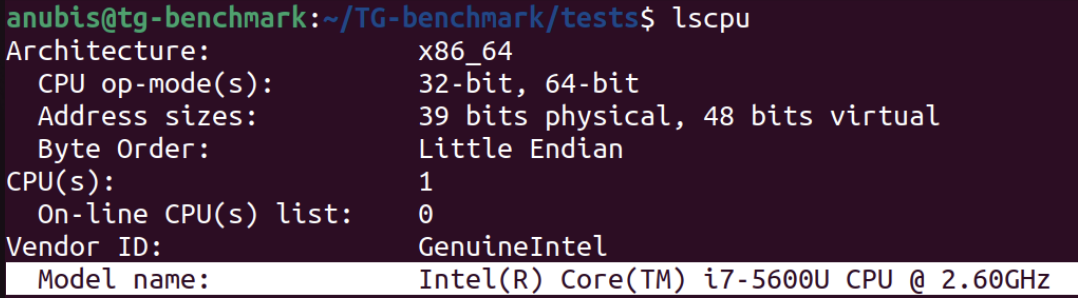
\includegraphics[width=\textwidth,height=0.85\textheight,keepaspectratio]{apendices/ENV-BENCH/CPU.png}
    \caption{CPU del entorno de \textit{benchmarking}}\label{fig:CPU-benchmarking}
\end{figure}

\noindent
En la Figura~\ref{fig:RAM-benchmarking} se muestra el estado de la memoria principal del entorno de \textit{benchmarking}, obtenido mediante el comando \texttt{free -h}. Se observa que el sistema cuenta con un total de 1.9 GiB de \RAM, de los cuales aproximadamente 572 MiB se encuentran en uso, mientras que 956 MiB permanecen libres. Adicionalmente, se dispone de 596 MiB utilizados por el sistema como memoria intermedia y de caché, dejando un total de 1.3 GiB disponibles para ejecución de procesos.
\begin{figure}[H]
    \centering
    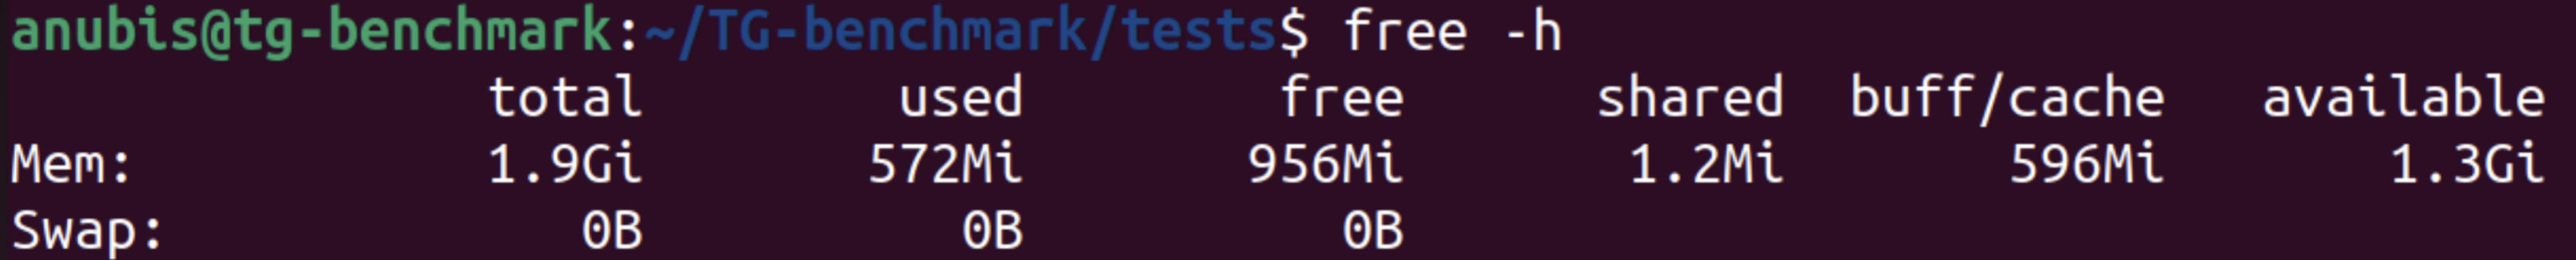
\includegraphics[width=\textwidth,height=0.85\textheight,keepaspectratio]{apendices/ENV-BENCH/RAM.png}
    \caption{RAM del entorno de \textit{benchmarking}}\label{fig:RAM-benchmarking}
\end{figure}
\noindent
En la Figura~\ref{fig:DISK-benchmarking} se presenta la información del sistema de archivos correspondiente al disco del entorno de \textit{benchmarking}, obtenida mediante el comando \texttt{df -Th}. El resultado muestra que el volumen principal está montado sobre el directorio raíz /, con un sistema de archivos ext4, una capacidad total de 14 GB, de los cuales 7.2 GB se encuentran en uso y 5.3 GB permanecen disponibles, lo que representa un 58\% de ocupación. Estos datos permiten evidenciar las características de almacenamiento del entorno, así como su disponibilidad para la ejecución de las pruebas experimentales sin limitaciones significativas de espacio.
\begin{figure}[H]
    \centering
    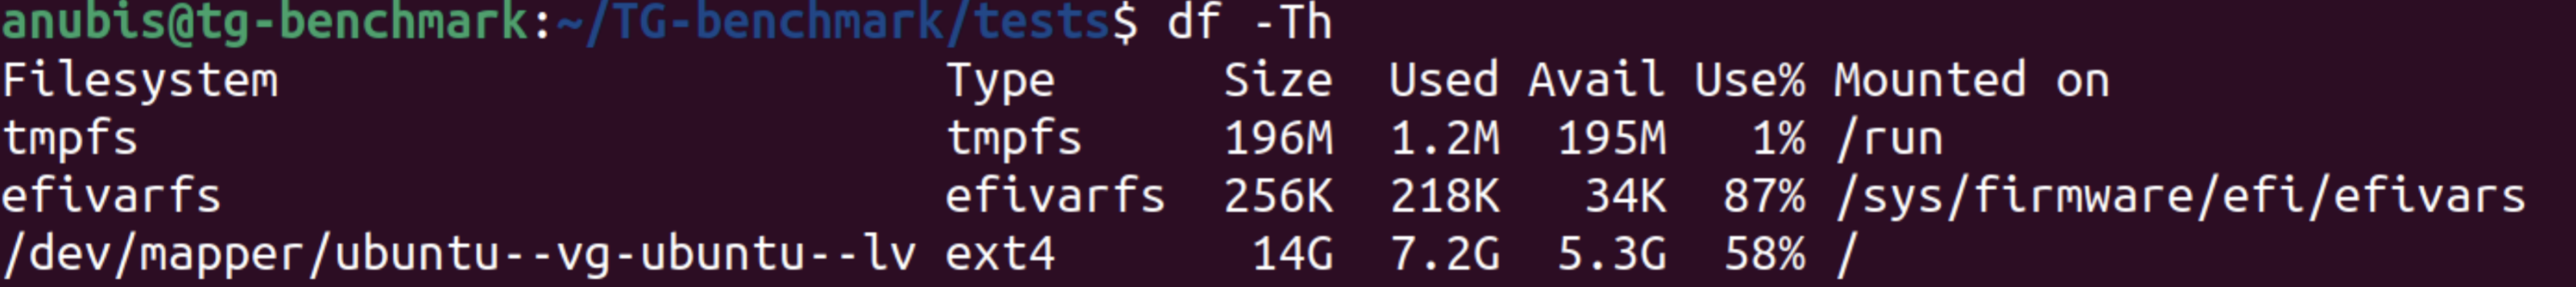
\includegraphics[width=\textwidth,height=0.85\textheight,keepaspectratio]{apendices/ENV-BENCH/DISCO.png}
    \caption{Disco del entorno de \textit{benchmarking}}\label{fig:DISK-benchmarking}
\end{figure}
\noindent
En la Figura~\ref{fig:OS-benchmarking} se presenta la información del sistema operativo empleado en el entorno de \textit{benchmarking}, obtenida mediante el comando \texttt{lsb\_release -a}. El resultado indica que se utiliza la distribución Ubuntu 24.04.2 LTS, cuyo nombre en clave es noble. Esta versión corresponde a una edición de soporte extendido (\textit{Long Term Support}), lo que ofrece estabilidad, actualizaciones de seguridad y mantenimiento a largo plazo. La elección de este sistema operativo resulta adecuada para la ejecución de pruebas experimentales, dado que proporciona un entorno ampliamente soportado en la comunidad de software libre.
\begin{figure}[H]
    \centering
    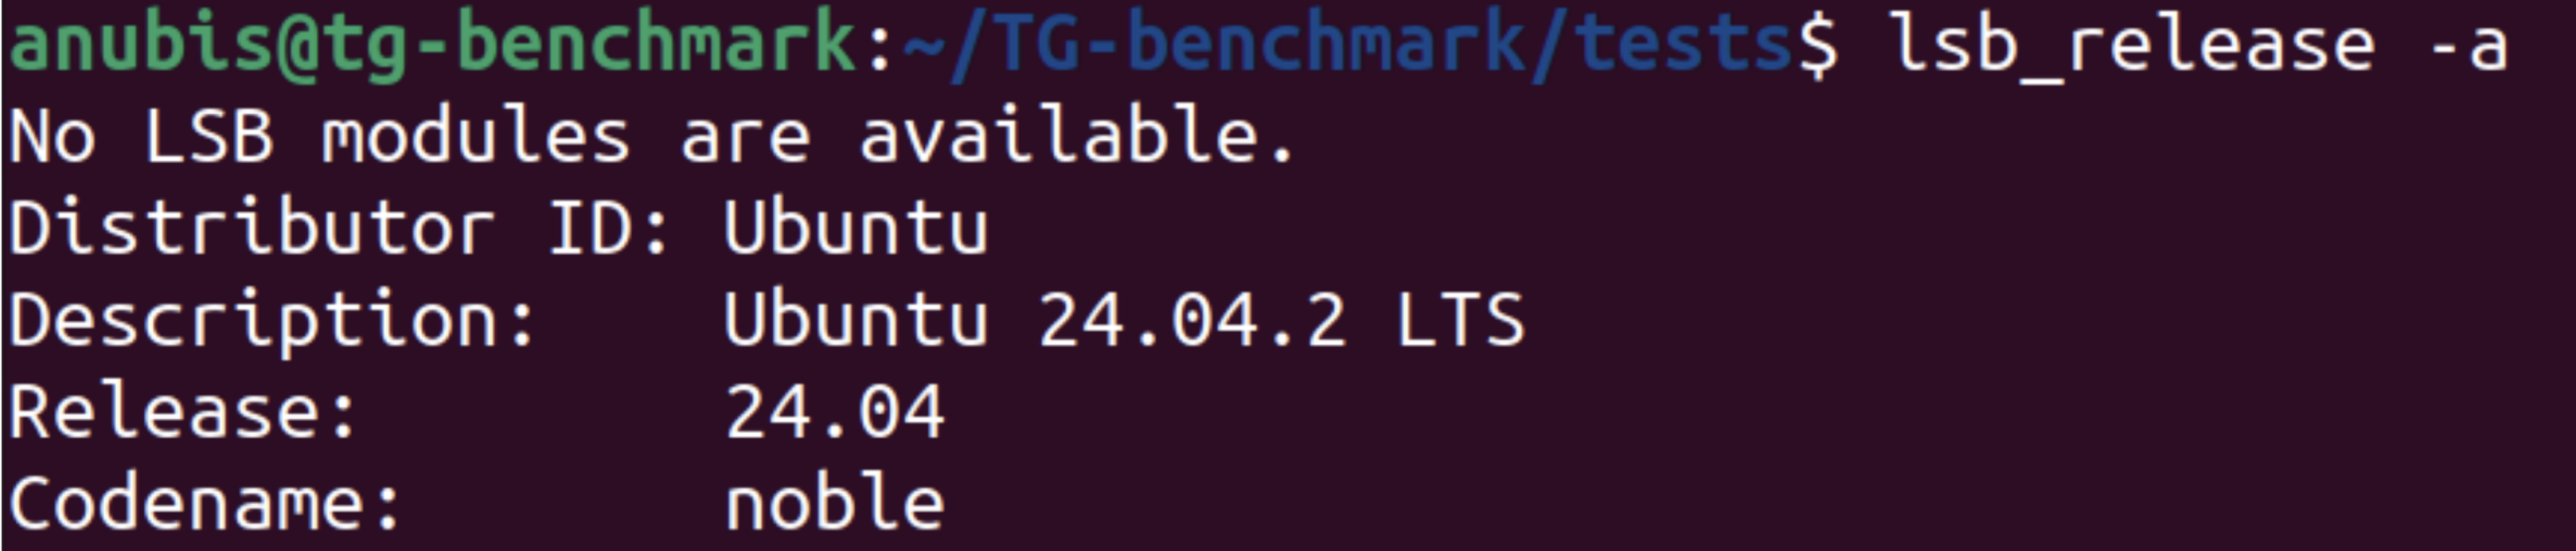
\includegraphics[width=\textwidth,height=0.85\textheight,keepaspectratio]{apendices/ENV-BENCH/OS.png}
    \caption{Sistema operativo del entorno de \textit{benchmarking}}\label{fig:OS-benchmarking}
\end{figure}
En la Figura~\ref{fig:INTERFACES-benchmarking} se muestra la configuración de las interfaces de red del entorno de benchmarking, obtenida mediante el comando \texttt{ip a}. Se identifican varias interfaces activas, entre ellas la \texttt{lo} (loopback) utilizada para la comunicación interna del sistema, así como \texttt{enp0s3} y \texttt{enp0s8}, ambas en estado operativo (UP) y con direcciones IPv4 asignadas en las subredes 10.0.2.0/24 y 192.168.0.0/24, respectivamente, además de direcciones IPv6 asociadas. También se observan interfaces virtuales, como \texttt{lxcbro} y \texttt{lxdbro}, que si bien aparecen en estado inactivo (DOWN), evidencian la presencia de configuraciones de red orientadas a entornos virtualizados. Esta información permite caracterizar la conectividad del sistema y su capacidad de interacción con diferentes redes dentro del proceso de evaluación de rendimiento.
\begin{figure}[H]
    \centering
    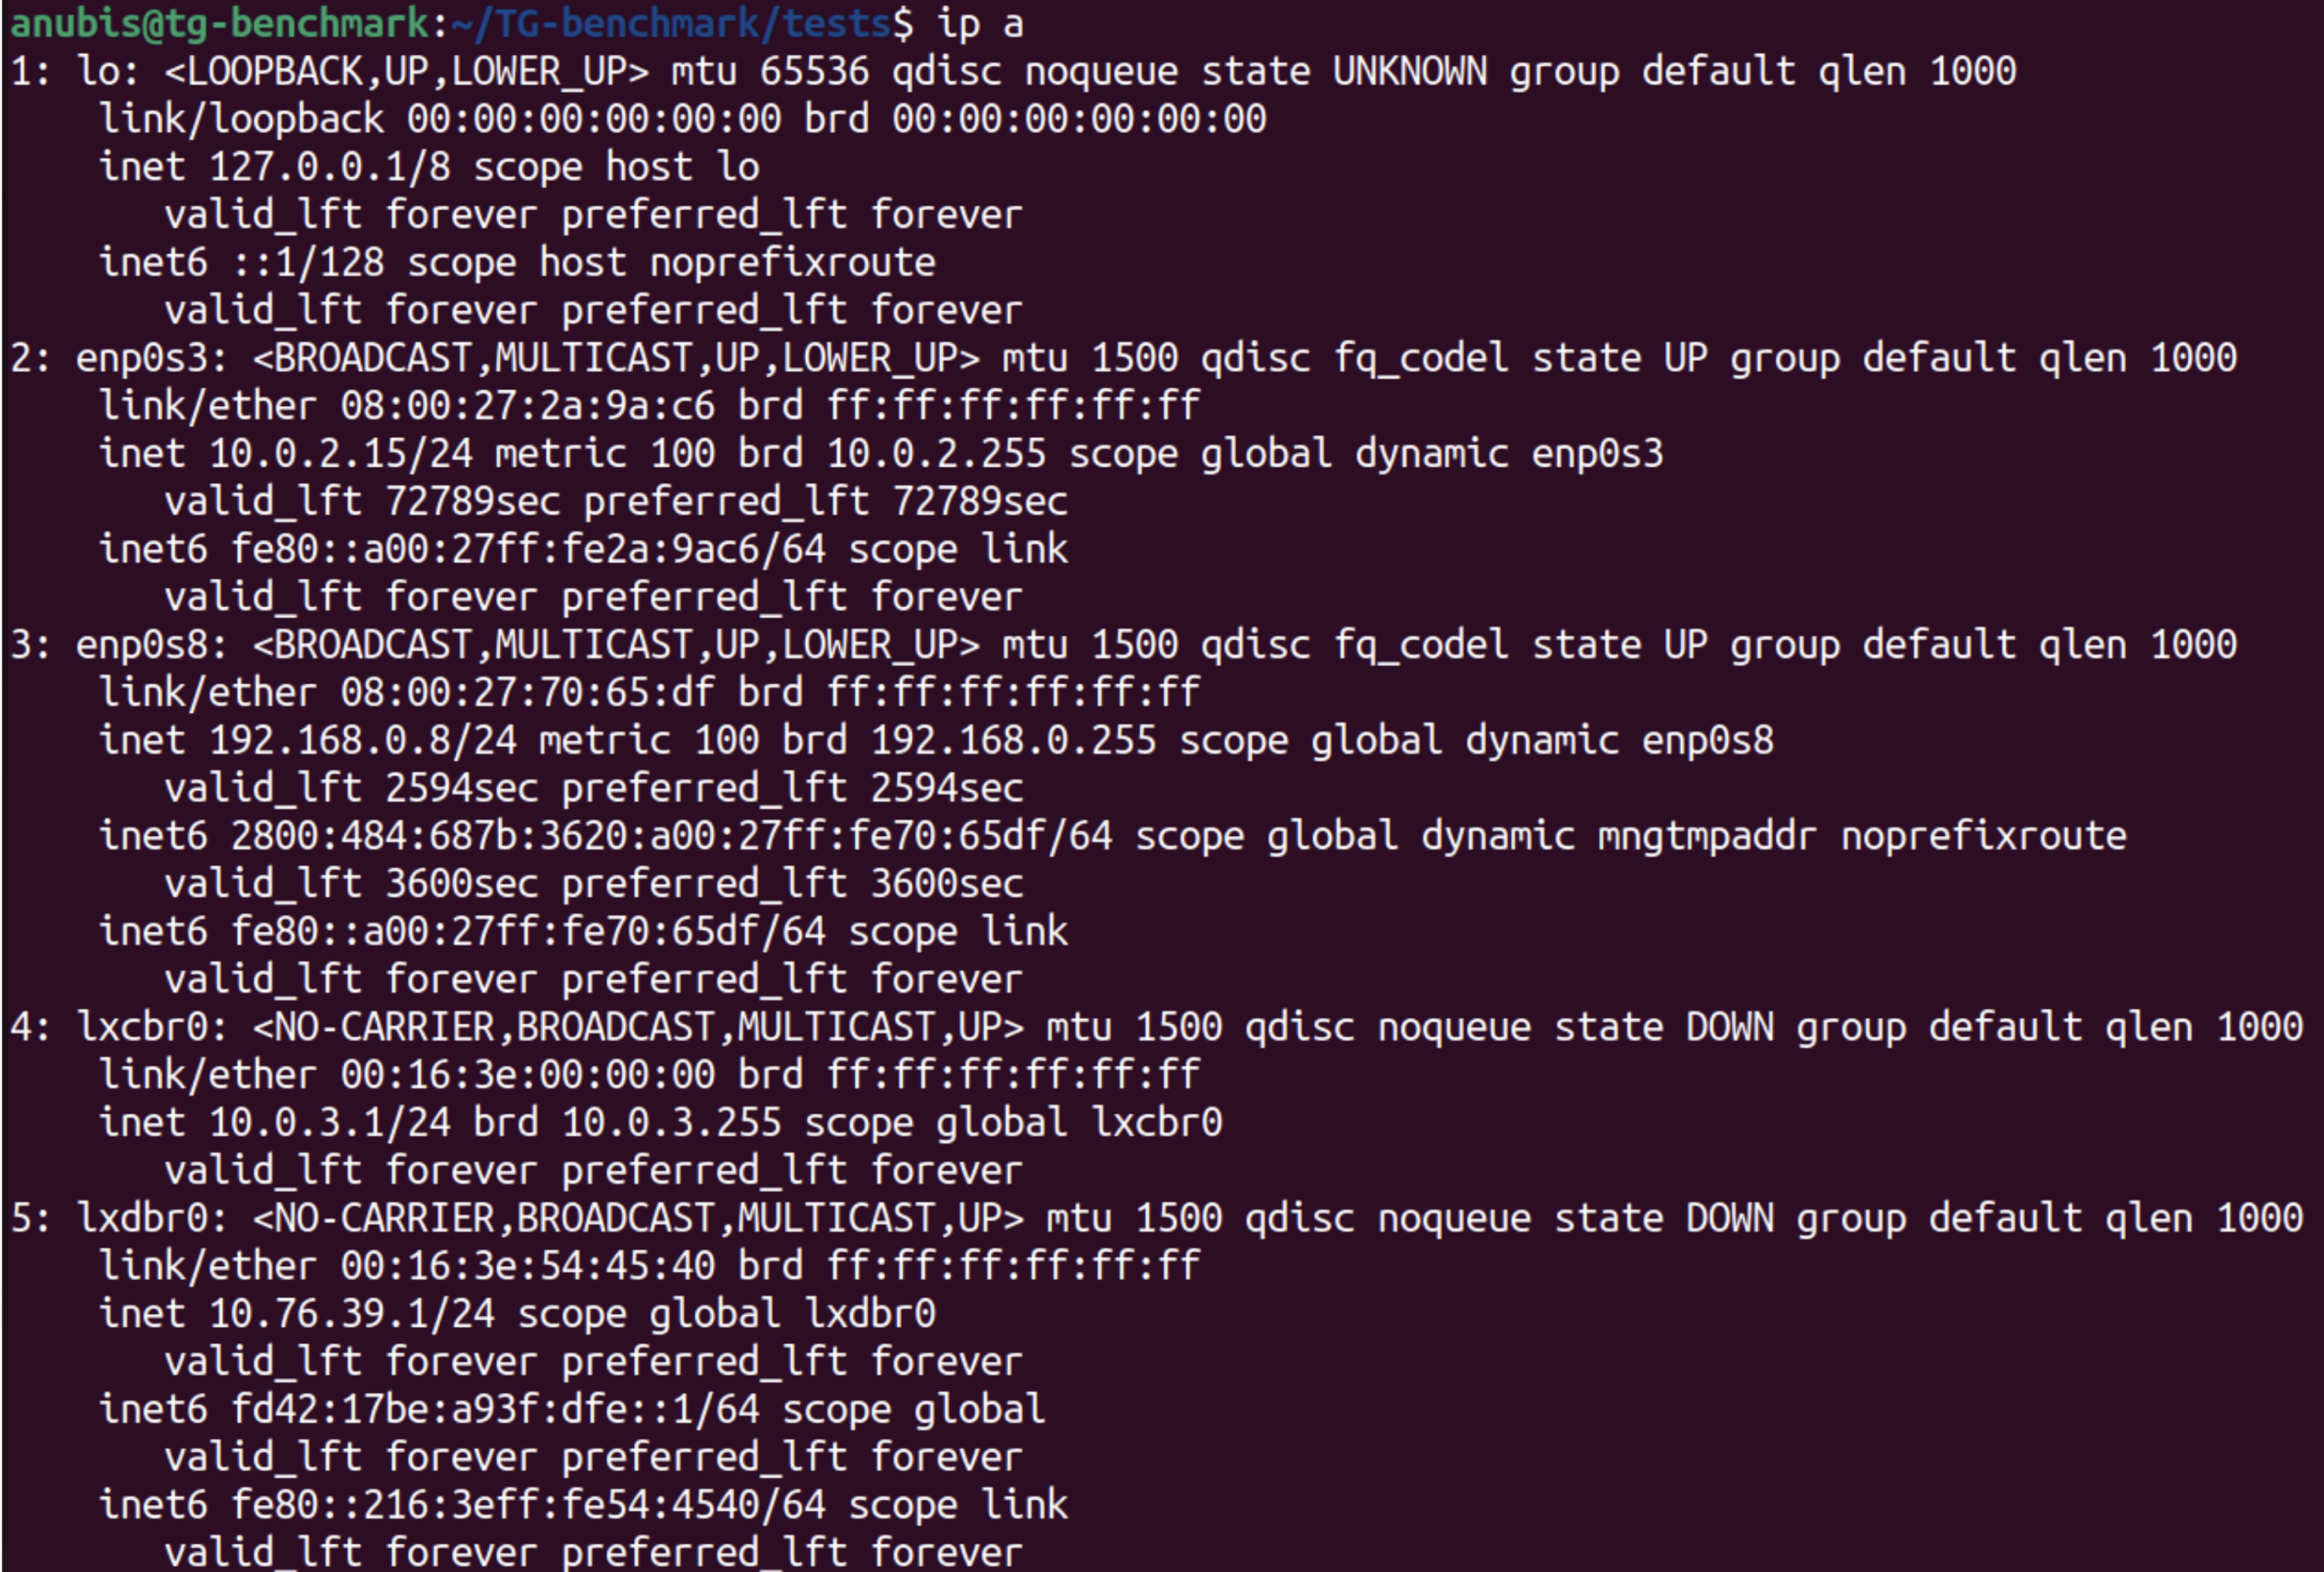
\includegraphics[width=\textwidth,height=0.85\textheight,keepaspectratio]{apendices/ENV-BENCH/interfaces.png}
    \caption{Interfaces de red del entorno de \textit{benchmarking}}\label{fig:INTERFACES-benchmarking}
\end{figure}

\section{Definición de las pruebas}
\noindent
Para evaluar el rendimiento de distintas tecnologías de contenerización —específicamente Docker, Podman, LXC, LXD y Containerd— se diseñó un conjunto de pruebas orientadas a medir aspectos clave del desempeño en entornos controlados. Las pruebas incluyeron el consumo de CPU y memoria RAM, el tiempo de arranque de los contenedores, el \textit{throughput} de red y la latencia de acceso a disco. 
Con el objetivo de facilitar la repetibilidad y objetividad de los resultados, se desarrollaron scripts en \textit{Bash} que automatizan la ejecución de cada métrica en condiciones homogéneas. Estas pruebas permiten comparar las tecnologías evaluadas bajo criterios cuantificables y facilitar un análisis técnico de sus capacidades en escenarios reales de uso.

\section{Construcción de las pruebas}
\noindent
La construcción de las pruebas se llevó a cabo mediante el desarrollo de scripts automatizados en \textit{Bash}, diseñados para ejecutarse de forma uniforme sobre cada tecnología de contenerización evaluada. Cada script fue responsable de iniciar contenedores, ejecutar cargas de trabajo específicas y recolectar métricas de rendimiento relevantes.
Para medir el consumo de \CPU\ y memoria \RAM, se utilizó \texttt{pidstat}, una utilidad que permite la medición del consumo de recursos. El tiempo de arranque se determinó midiendo el intervalo entre la orden de inicio del contenedor y el momento en que estuvo completamente operativo. 
Para evaluar el \textit{throughput} de red se emplearon herramientas como \texttt{iperf}, mientras que la latencia de disco fue medida utilizando \texttt{fio}. Todas las pruebas fueron ejecutadas múltiples veces para reducir el impacto de variaciones puntuales y asegurar la confiabilidad de los resultados. Los scripts fueron programados para ejecutarse 10 veces; al final se extrae un promedio y este constituye el puntaje final de la tecnología de contenerización en cuestión.
En el repositorio \underline{\href{https://github.com/Anubis-1001/benchmark-tecnologias-de-contenerizacion} {\texttt{ GitHub benchmarking}}} se pueden encontrar los scripts resultantes de este proceso.

\section{Resultados de las pruebas}
\noindent
Los resultados obtenidos a partir de las pruebas evidencian diferencias significativas en el rendimiento entre las tecnologías de contenerización evaluadas. Estos se pueden consultar en el archivo de Excel \underline{\href{https://docs.google.com/spreadsheets/d/1Ce37Sm3Swyfa88Ur1yQbLarq_D86obUIAGGJocgQbUE/edit?usp=sharing} {\texttt{benchmarking\_tecnologias}}}.
En términos de consumo de \CPU, Docker y Containerd presentan las mejores métricas; en consumo de memoria \RAM, LXC y LXD mostraron un mejor uso de los recursos. En cuanto al tiempo de arranque, Containerd destacó por su velocidad, seguido de cerca por Docker, mientras que LXC presentó un arranque considerablemente más lento en comparación con las demás tecnologías.
Para el \textit{throughput} de red, todas las tecnologías mostraron un desempeño comparable, siendo LXC el más destacado; no obstante, Podman quedó muy por debajo en esta métrica. Finalmente, en la medición de latencia de disco, LXD y Containerd obtuvieron los mejores resultados, lo que sugiere una gestión de E/S más directa y liviana.
Estos resultados permiten establecer un panorama claro de fortalezas y debilidades de cada solución, según el tipo de carga o entorno de ejecución esperado.

\section{Métricas de rendimiento}
\noindent
De la ejecución de las pruebas se obtuvieron las siguientes métricas de rendimiento: \\

\noindent
La figura~\ref{fig:tabla-metricas-cpu} muestra una comparación del porcentaje de uso de \CPU. Este análisis permite observar el nivel de utilización del procesador al ejecutar cargas de trabajo bajo entornos como Docker, Containerd, LXD, LXC y Podman. Los resultados tienen contrastes significativos entre las tecnologías, destacando aquellas que logran un mayor aprovechamiento del recurso de CPU frente a otras con un desempeño relativamente inferior.
\begin{figure}[H]
    \centering
    \includegraphics[width=\textwidth] {tablas-images/cp4/cpu.png}
    \caption{Métricas de uso de CPU}\label{fig:tabla-metricas-cpu}
\end{figure}

\noindent
La figura~\ref{fig:tabla-metricas-ram} presenta una comparación del porcentaje de uso de memoria \RAM para el conjunto de tecnologías seleccionado. Este análisis permite evaluar el consumo de recursos de cada solución, considerando que un menor uso de memoria representa una ventaja en términos de escalabilidad y rendimiento en entornos de alta demanda. Los resultados muestran valores muy cercanos entre las tecnologías evaluadas, lo que sugiere un comportamiento homogéneo en este aspecto, aunque con ligeras variaciones que pueden influir en la elección según el contexto de uso.
\begin{figure}[H]
    \centering
    \includegraphics[width=\textwidth] {tablas-images/cp4/ram.png}
    \caption{Métricas de uso de RAM}\label{fig:tabla-metricas-ram}
\end{figure}

\noindent
La figura~\ref{fig:tabla-metricas-io} muestra las métricas de latencia en operaciones de entrada/salida (E/S) para el conjunto de tecnologías seleccionado, expresadas en microsegundos. Este indicador es fundamental para evaluar el rendimiento de aplicaciones que dependen de un acceso rápido a datos y procesos intensivos en E/S. Los resultados reflejan diferencias significativas entre las tecnologías, evidenciando desde valores muy bajos, como en LXD, hasta tiempos de respuesta considerablemente altos, como en Podman. Este contraste permite identificar cuáles soluciones resultan más adecuadas en escenarios donde el manejo de datos es un factor crítico.
\begin{figure}[H]
    \centering
    \includegraphics[width=\textwidth] {tablas-images/cp4/io.png}
    \caption{Métricas de entrada/salida}\label{fig:tabla-metricas-io}
\end{figure}

\noindent
La figura~\ref{fig:tabla-metricas-throughput} presenta una comparación de las métricas de throughput (rendimiento de transferencia de datos) para el conjunto de tecnologías seleccionado, expresadas en Gbits por segundo. Este parámetro resulta clave para evaluar la capacidad de cada tecnología en la transmisión de información a través de la red, lo cual impacta directamente en el desempeño de aplicaciones distribuidas y servicios en la nube. Los resultados muestran un rendimiento consistente en tecnologías como LXC, LXD, Docker y Containerd, mientras que Podman evidencia un throughput significativamente más bajo, lo que resalta contrastes importantes en términos de consumo de red
\begin{figure}[H]
    \centering
    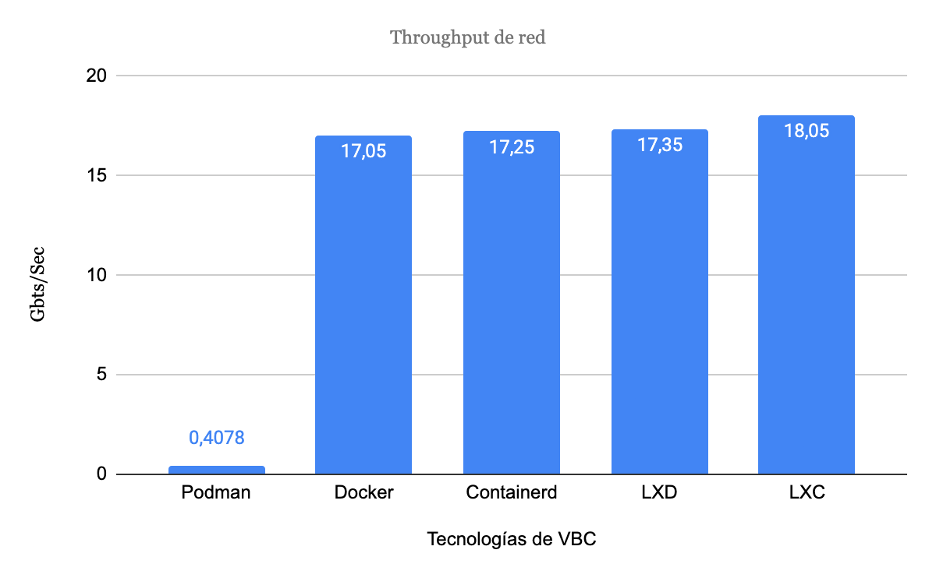
\includegraphics[width=\textwidth] {tablas-images/cp4/THROUGHTPUT.png}
    \caption{Métricas de throughput}\label{fig:tabla-metricas-throughput}
\end{figure}

\section{Análisis de los resultados}
\noindent
Los resultados obtenidos a partir de las pruebas permiten identificar comportamientos diferenciados entre las tecnologías de contenerización evaluadas. Containerd se posiciona como una de las soluciones más equilibradas, con excelente tiempo de arranque, bajo uso de CPU y buena latencia de disco, lo que lo hace ideal para entornos de bajos recursos.
LXC mostró consistentemente el menor consumo de recursos y alto rendimiento en red, lo que lo convierte en una opción adecuada para sistemas embebidos o despliegues que requieren un uso mínimo de \textit{overhead}. 
Por otro lado, Docker ofreció un rendimiento aceptable, pero con mayores niveles de consumo de CPU y latencia de disco, compensados por su madurez y ecosistema. 
LXD, al estar basado en LXC, heredó parte de sus beneficios, especialmente en uso de red, aunque con un ligero incremento en el tiempo de arranque.
En contraste, Podman, si bien ofrece un buen uso de CPU y memoria, presentó resultados considerablemente bajos en el \textit{throughput} de red y alta latencia de disco, lo cual podría limitar su aplicación en cargas sensibles a E/S o comunicación intensiva.

\vspace{0.5em}

\noindent En resumen, la elección de la tecnología de contenerización debe considerar el caso de uso específico: Containerd y LXC sobresalen por su bajo consumo de recursos; Docker y LXD ofrecen robustez y facilidad de integración; mientras que Podman puede ser más adecuado para entornos que prioricen la seguridad y compatibilidad con el modelo sin \textit{daemon}, siempre que el rendimiento de red o disco no sea crítico.
